\documentclass[11pt,a4paper]{article}
\usepackage[margin=22mm]{geometry}
\usepackage{fontspec,amsmath,booktabs,graphicx,hyperref}
\setmainfont{STIXGeneral}
\setlength{\emergencystretch}{2em}
\begin{document}
\begin{center}{\Large Topic C: common theory, applications and required code}\\[4pt]
Human Compression project\end{center}
The common paper \emph{Changes of chamber generators and binary translation
groups} supports four complete applications: Janko geometries (C1), halving
generalized cubes (C2), Petrials and faithful chamber actions (C3), and regular
polyhedra with equal adjacent parameters (C4). The fixed source contracts
are L088, N013, L108 and F014. Their forty-row scope table includes the
recorded qualifications, retained statements and exclusions; this
measurement does not expand that scope.

\paragraph{The complete topic.}
The whole common theory costs \textbf{27,131} characters. The four complete
applications cost \textbf{44,146}, and the complete printed appendix of both
required programs costs \textbf{8,799}. Charging each once gives
\textbf{80,076}. The three available source PDFs cost 60,256. If $x$ is the
unknown original-PDF cost of L108, the complete comparison is
\[R_C=\frac{x+60\,256}{80\,076}.\]
No numerical value of $R_C$ is available. C3's 10,071 characters remain in
the denominator. Its authored browser text is not substituted for the missing PDF.

\begin{center}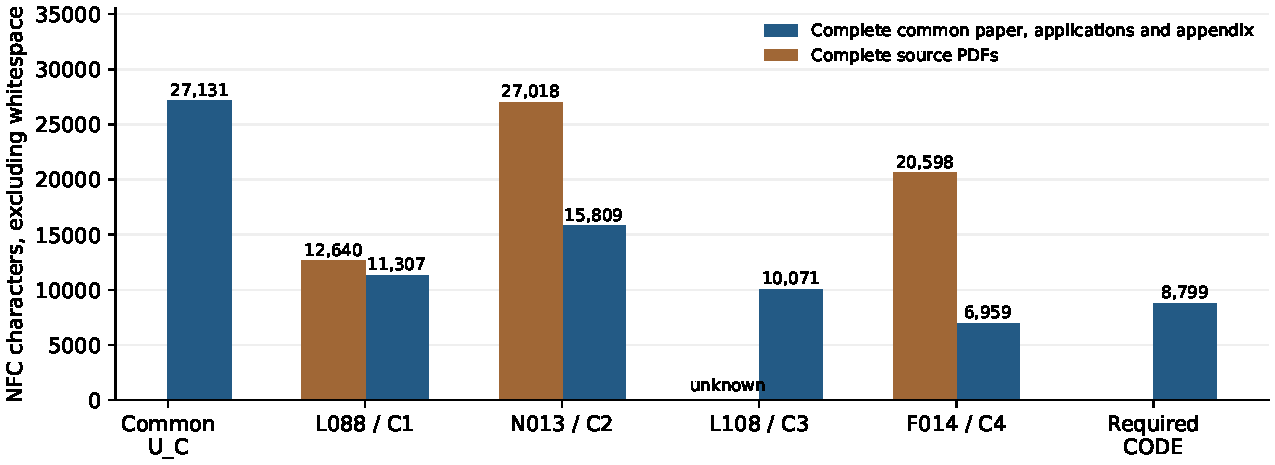
\includegraphics[width=\linewidth]{costs.pdf}\end{center}
\noindent These are NFC characters without whitespace in complete extracted
PDF text, after the exact furniture exclusions and visible-glyph corrections.
All unique front matter and references remain charged.

\paragraph{Conditional application comparisons.}
After acquiring the \emph{whole common theory and both complete required
programs}, the local comparison is the complete source paper divided by its
complete application. The overall denominator above pays the common work once.
\begin{center}\begin{tabular}{lrrr}\toprule
Source / application & Source & Application & Conditional factor\\\midrule
L088 / C1 & 12,640 & 11,307 & 1.118\\
N013 / C2 & 27,018 & 15,809 & 1.709\\
L108 / C3 & unknown & 10,071 & unknown\\
F014 / C4 & 20,598 & 6,959 & 2.960\\
\bottomrule\end{tabular}\end{center}
\newpage
\paragraph{The code is counted once, in a declared representation.}
Both GAP files are required mathematical programs and are charged in full.
The primary representation is their four-page printed appendix, including
its headings and printed glyphs. An alternative uses the complete raw files:
4,458 and 4,783 bytes, with 4,084 and 4,239 NFC nonspace characters.
The alternative replaces the appendix; it is never added to it.
\begin{center}\begin{tabular}{p{.64\linewidth}r}\toprule
Denominator representation & NFC nonspace cost\\\midrule
Common paper and four applications only & 71,277\\
Complete topic with printed program appendix (primary) & 80,076\\
Complete topic with both raw programs (alternative) & 79,600\\\bottomrule
\end{tabular}\end{center}
All three numerators remain $x+60\,256$. The papers-only coordinate is a
separately labeled sensitivity, not the complete required-cost comparison.
The raw-file metrics are summed file by file; no program or diagnostic
portion is pruned. There is no cross-topic discount on the common theory.

\paragraph{What was measured.}
The source inputs are three complete physical PDFs, totaling 33 pages.
The new side consists of the complete 27-page scientific edition and the
four-page required-program appendix. Only exact running furniture and
navigation are excluded. Font-aware glyph replacements precede Unicode
normalization; no semantic correction, dehyphenation, formula reordering or
coalescing of printed delimiter pieces is performed.

The machine-readable record contains all five length units under NFC and
NFKC, for raw untrimmed, raw selected and calibrated selected text. Each of
these thirty coordinates has the same full denominator boundary and the
three declared program representations. Exact conditional fractions appear
in the CSV and JSON files. The primary coordinate is the calibrated NFC
nonspace count used on page one.

\paragraph{Scope and retained work.}
The Janko application keeps the accepted figure/label qualification. The
halving application retains its qualified statement and excludes the
specified external-classification comparison and unused semiregular
isomorphism. For L108, the unconditional faithful-action assertion is
replaced by the exact kernel criterion. F014 uses the fixed first edition
and corrected left-action convention; its higher-rank Conjecture 3.7 belongs
to the separate question track.

The TomLib subgroup catalogue, group and coset algorithms, Danzer and
Pellicer constructions, Coxeter classifications and other stated classical
inputs remain attributed and retained. Their expanded proof and catalogue
costs are unknown, as are unextracted graphical and formula-layout costs.
The extracted-text comparison is not a measurement of total research effort
or minimum mathematical complexity.

\paragraph{Verification and use.}
The independently accepted input audit matches 270 PDF metric cells,
54 normalized-text hashes and 20 complete raw-program cells. It checks the
embedded fonts and visible glyph conventions. This numerical packet reuses
that acceptance and computes only sums, exact fractions and CSV records;
it does not repeat the source, GAP or Lean proof work. The 16 scoped Lean
declarations and other validation infrastructure remain separately
inventoried, without a claim that every application is fully formalized.

Reproduce the arithmetic with \texttt{compute.py --out /fresh/directory};
\texttt{check.py} verifies the complete boundary, both code representations,
all coordinate records and corruption controls. No primary-source text or
images are distributed. Independent arithmetic and reader review is separate
from this author calculation. No source or question credit is added.
\end{document}
